\PassOptionsToPackage{quiet}{fontspec}
\documentclass[12pt,a4paper]{article}
\usepackage{thesis} % 格式控制
\usepackage{indentfirst}
\usepackage{enumitem}
\usepackage{amsmath} % 数学公式支持
\usepackage{amsfonts} % 数学字体支持
\usepackage{amssymb} % 数学符号支持
\usepackage{graphicx} % 图片插入支持
\usepackage{float} % 浮动体位置控制，支持 [H] 选项
\usepackage{caption} % 图表标题格式控制
\usepackage{geometry} % 页面布局控制
\usepackage{setspace} % 行距控制
\usepackage{xeCJK} % 中文字体支持
\usepackage{fontspec} % 字体设置
\usepackage[most]{tcolorbox} % 高亮按键命令
\usepackage{listings} % 代码高亮
\usepackage[table]{xcolor} % 颜色支持
\setlength{\parindent}{2em} % 控制首行缩进  
\addtolength{\parskip}{3pt} % 控制段落距离  
\onehalfspacing % 1.5倍行距  
\graphicspath{{./figures/}} % 指定图片所在文件夹  
\setCJKmainfont{SimSun}

% 配置lstlisting样式
\lstset{
    basicstyle=\ttfamily\small,
    breaklines=true,
    frame=single,
    numbers=left,
    numberstyle=\tiny\color{gray},
    backgroundcolor=\color{gray!10},
    keywordstyle=\color{blue},
    commentstyle=\color{green!60!black},
    stringstyle=\color{red},
    showstringspaces=false,
    tabsize=4,
    captionpos=b,
    xleftmargin=2em,
    xrightmargin=2em,
    aboveskip=1em,
    belowskip=1em
}

\classname{\heiti\bfseries 信息电子学物理基础}  % 设置课程名称
\makepagestyle{}{}

\newtcbox{\keyblue}{on line,
  colframe=blue!60!black, colback=blue!5,
  boxrule=0.8pt, arc=2pt, boxsep=0pt, left=3pt, right=3pt, top=2pt, bottom=2pt,
  tcbox raise base, fontupper=\ttfamily\small}

\newtcbox{\pathbox}{on line,
  colframe=green!60!black, colback=green!5,
  boxrule=0.8pt, arc=2pt, boxsep=0pt, left=3pt, right=3pt, top=2pt, bottom=2pt,
  tcbox raise base, fontupper=\ttfamily\small}

\begin{document}
\maketitlepage{量子点发光智能服装设计}{玉泉教7-104}{}{}{\today}{林时胜} %封面页 

\maketoc

\section{设计指标与要求}

设计一个 pn 结，工作温度为 $T = 300\,\text{K}$，需满足以下技术指标：

\begin{itemize}[leftmargin=2em]
    \item 开启电压小于 $0.800\,\text{V}$；
    
    \item 正偏时，空穴与电子对电流的贡献相同；
    
    \item 反偏为 $5\,\text{V}$ 时，结电容小于 $1.60 \times 10^{-9}\,\text{F/cm}^2$；
    
    \item 反偏时，电流密度小于 $1.30 \times 10^{-8}\,\text{A/cm}^2$。
\end{itemize}

\vspace{0.5em}
\noindent 可选的设计材料及其参数如下：

\begin{table}[H]
\centering
\caption{可选材料的少数载流子寿命}
\label{tab:minority_lifetime}
\begin{tabular}{|c|c|c|c|}
\hline
{\heiti 材料} & \textbf{Si} & \textbf{Ge} & \textbf{GaAs} \\
\hline
少数载流子寿命 ($\mu$s，少子 = 空穴) & 10 & 200 & $5 \times 10^{-3}$ \\
\hline
\end{tabular}
\end{table}

\clearpage
\section{PN结设计}
\subsection{材料选择}

根据设计指标要求，需要对三种候选材料（Ge、GaAs、Si）进行系统性评估。评估过程主要考虑以下四个关键参数：开启电压、漏电流密度、少数载流子寿命以及对传输效率的影响。

\subsubsection{开启电压分析}

开启电压是 pn 结的重要特性参数，直接影响器件的工作电压范围。根据设计要求，开启电压需小于 $0.800\,\text{V}$。三种材料的开启电压特性如下：

\begin{itemize}[leftmargin=2em]
    \item {\heiti Ge（锗）}：开启电压约为 $0.3\,\text{V}$，满足设计要求；
    \item {\heiti GaAs（砷化镓）}：开启电压约为 $1.2\,\text{V}$，超出设计指标，不符合要求；
    \item {\heiti Si（硅）}：开启电压范围为 $0.6\sim0.7\,\text{V}$，满足设计要求。
\end{itemize}

\begin{figure}[H]
\centering
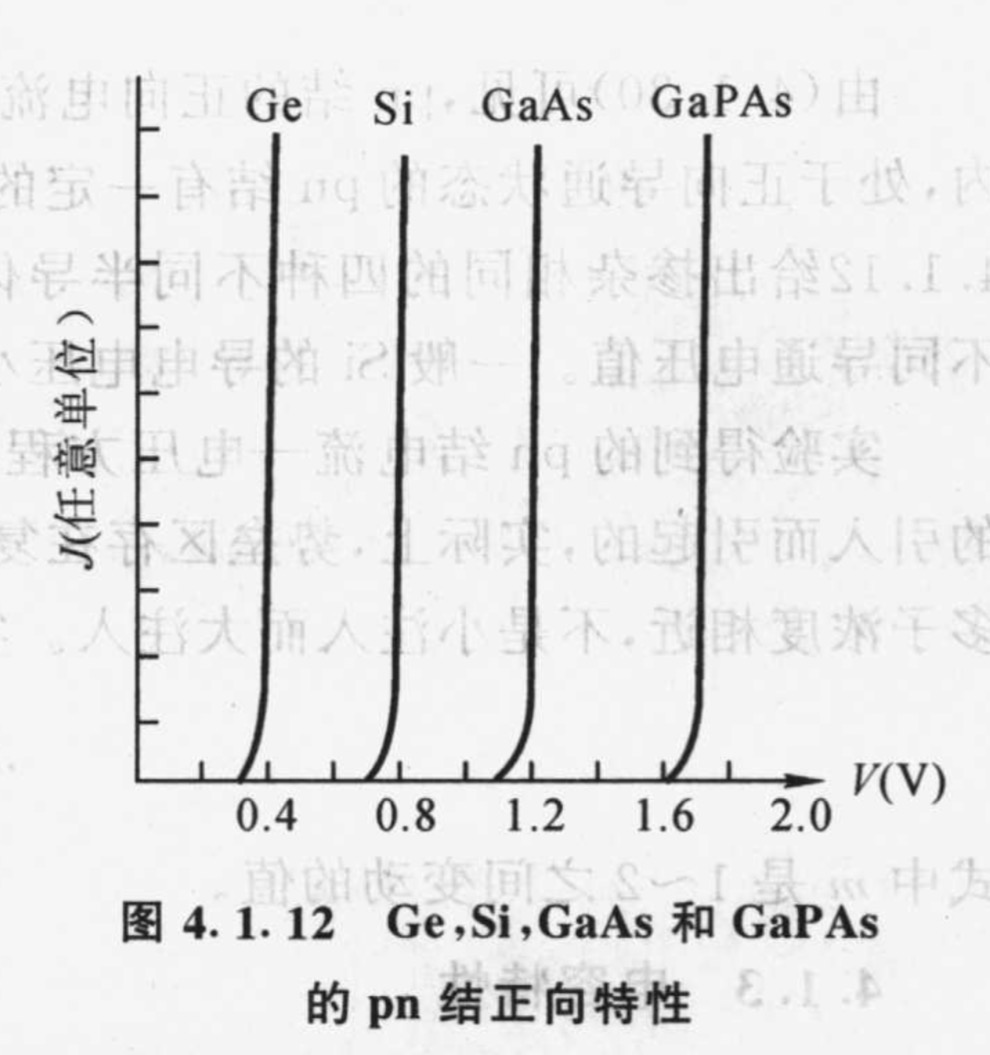
\includegraphics[width=0.6\textwidth]{p1.jpg}
\caption[不同半导体材料的开启电压特性]{不同半导体材料的开启电压特性\footnotemark}
\label{fig:p1}
\end{figure}

\footnotetext{杨东晓, 陈秀峰. 现代信息电子学物理[M].}

\subsubsection{漏电流特性分析}

反向偏置下的漏电流密度需小于 $13\,\text{nA/cm}^2$（即 $1.30 \times 10^{-8}\,\text{A/cm}^2$）。

由于反向饱和电流密度 $J_0$ 与材料本征载流子浓度 $n_i$ 的平方成正比关系：
\begin{equation}
J_0 \propto n_i^2
\end{equation}

因此，本征载流子浓度的高低直接决定了反向漏电流的大小。

\begin{itemize}[leftmargin=2em]
    \item {\heiti Ge（锗）}：在 $T = 300\,\text{K}$ 时，Ge 的本征载流子浓度 $n_i \approx 2.4 \times 10^{13}\,\text{cm}^{-3}$，远高于其他材料。由于 $n_i$ 极高，Ge 二极管的漏电流通常在 $\mu\text{A}$ 级别，比设计要求的 $\text{nA}$ 级别高出约 3 个数量级（1000 倍以上），根本无法满足 $13\,\text{nA/cm}^2$ 的严苛限制；

    \item {\heiti GaAs（砷化镓）}：漏电流极小，符合设计指标；

    \item {\heiti Si（硅）}：在 $T = 300\,\text{K}$ 时，$n_i \approx 1.5 \times 10^{10}\,\text{cm}^{-3}$。相比 Ge，其 $n_i^2$ 低了约 6 个数量级。Si 二极管的理论漏电流可轻松控制在 $\text{pA} \sim \text{nA}$ 级别，完全符合设计指标。
\end{itemize}

\subsubsection{少数载流子寿命分析}

少数载流子寿命直接影响载流子的传输效率和器件性能。根据设计要求，少数载流子寿命参数必须适宜常规 pn 结设计。

{\heiti 材料对比分析：}

\begin{itemize}[leftmargin=2em]
    \item {\heiti GaAs（砷化镓）}：寿命为 $5 \times 10^{-3}\,\mu\text{s}$（即 $5\,\text{ns}$），极短的寿命意味着复合率极高。虽然这适合超高速开关应用，但在常规整流或低频应用中，过短的寿命会导致正向导通时的压降增大（电导调制效应减弱），不利于载流子有效扩散；
    
    \item {\heiti Ge（锗）}：寿命为 $200\,\mu\text{s}$，虽然长寿命利于载流子扩散，但结合前述的高漏电流特性，这种长寿命会导致反向恢复时间变慢，且无法弥补其漏电缺陷；
    
    \item {\heiti Si（硅）}：寿命为 $10\,\mu\text{s}$，是一个非常均衡的数值。它既足够长，保证了正向偏置时少子能有效扩散（满足电流方程的理论假设），又没有过短导致复合损耗过大。这使得利用标准扩散理论计算掺杂浓度 $N_a$ 和 $N_d$ 变得准确且可控。
\end{itemize}

{\heiti 结论：}Si 的载流子寿命参数最适合本设计的工作条件。

\subsubsection{结电容与掺杂浓度的可实现性分析}

根据设计指标，反偏 $5\,\text{V}$ 时，结电容需满足 $C_j < 1.60 \times 10^{-9}\,\text{F/cm}^2$。结电容与掺杂浓度密切相关，是评估材料工艺可行性的重要维度。

{\heiti 物理机理：}

低电容要求意味着耗尽层必须较宽，这需要较低的掺杂浓度（经理论计算约为 $10^{14}\,\text{cm}^{-3}$ 量级）。结电容与耗尽层宽度成反比，而耗尽层宽度与掺杂浓度的平方根成反比。

{\heiti 材料工艺分析：}

\begin{itemize}[leftmargin=2em]
    \item {\heiti Si（硅）}：在硅中，控制 $10^{14}\,\text{cm}^{-3}$ 的轻掺杂是标准成熟工艺，且在此掺杂浓度下，硅的电阻率适中，不会导致过大的串联电阻。Si 在平衡"低漏电"和"低电容"这两个相互制约的指标上，具有最佳的材料特性窗口；
    
    \item {\heiti Ge（锗）}：如果为了降低 Ge 的漏电流而强行提高掺杂浓度，会导致耗尽层变薄，结电容急剧增大，从而违反电容指标。因此 Ge 无法同时满足低漏电和低电容的要求；
    
    \item {\heiti GaAs（砷化镓）}：虽然可以通过掺杂控制电容，但其开启电压过高和少子寿命过短的缺陷已将其排除。
\end{itemize}

{\heiti 结论：}Si 材料允许在低掺杂下同时满足电容要求和漏电流要求，且工艺成熟可控。

\subsubsection{综合评估}

综合考虑上述四个维度的分析结果，对三种材料的适用性进行评估：

\begin{itemize}[leftmargin=2em]
    \item {\heiti Ge（锗）}：虽然开启电压较低，但本征载流子浓度过高导致漏电流严重超标（达 $\mu\text{A}$ 级别），且无法通过掺杂优化同时满足低漏电和低电容的要求，不适合作为设计材料；
    
    \item {\heiti GaAs（砷化镓）}：开启电压过高（约 $1.2\,\text{V}$）且少子寿命过短（$5\,\text{ns}$），两项关键指标均不满足要求，淘汰；
    
    \item {\heiti Si（硅）}：开启电压适中（$0.6\sim0.7\,\text{V}$），漏电流可控（$\text{pA}\sim\text{nA}$ 级别），少子寿命均衡（$10\,\mu\text{s}$），且在低掺杂下可同时满足电容和漏电要求，工艺成熟。所有指标均满足设计要求，且性能参数均衡合理，是最佳选择。
\end{itemize}

因此，{\heiti 选择Si（硅）作为 pn 结的半导体材料}。

\begin{table}[H]
\centering
\caption{三种候选材料的性能对比分析}
\label{tab:material_comparison}
\begin{tabular}{|c|c|c|c|c|}
\hline
\rowcolor{gray!20}
{\heiti 考量维度} & {\heiti 指标要求} & {\heiti Ge（锗）} & {\heiti GaAs（砷化镓）} & {\heiti Si（硅）} \\
\hline
开启电压 & $< 0.800\,\text{V}$ & \cellcolor{green!20}{\checkmark} ($< 0.3\,\text{V}$) & \cellcolor{red!20}{\texttimes} ($\sim 1.2\,\text{V}$) & \cellcolor{green!20}{\checkmark} ($0.6\sim0.7\,\text{V}$) \\
\hline
漏电流 & $< 13\,\text{nA/cm}^2$ & \cellcolor{red!20}{\texttimes} （过大，$\mu$A级） & \cellcolor{green!20}{\checkmark} （极小） & \cellcolor{green!20}{\checkmark} （符合，nA/pA级） \\
\hline
少子寿命 & 影响传输效率 & $200\,\mu\text{s}$ & $0.005\,\mu\text{s}$ （过短） & $10\,\mu\text{s}$ （均衡） \\
\hline
\rowcolor{gray!10}
{\heiti 结论} & & 淘汰 & 淘汰 & {\heiti 最佳选择} \\
\hline
\end{tabular}
\end{table}

\clearpage
\subsection{参数设计}

\subsubsection{物理常数与设计参数设定}

在进行 pn 结参数设计之前，需要确定工作温度 $T = 300\,\text{K}$ 下硅材料的物理常数和材料参数。这些参数是后续计算的基础。

\begin{table}[H]
\centering
\caption{硅材料在 $T = 300\,\text{K}$ 时的物理常数与材料参数}
\label{tab:si_parameters}
\begin{tabular}{|l|c|c|}
\hline
\rowcolor{gray!20}
{\heiti 参数名称} & {\heiti 符号} & {\heiti 数值} \\
\hline
本征载流子浓度 & $n_i$ & $1.5 \times 10^{10}\,\text{cm}^{-3}$ \\
\hline
真空介电常数 & $\epsilon_0$ & $8.85 \times 10^{-14}\,\text{F/cm}$ \\
\hline
硅相对介电常数 & $\epsilon_r$ & $11.7$ \\
\hline
电子电荷量 & $e$ & $1.602 \times 10^{-19}\,\text{C}$ \\
\hline
玻尔兹曼常数 & $k_B$ & $1.38 \times 10^{-23}\,\text{J/K}$ \\
\hline
热电压 & $V_T = k_B T / e$ & $0.02585\,\text{V}$ \\
\hline
电子扩散系数 & $D_n$ & $34.93\,\text{cm}^2/\text{s}$ \\
\hline
空穴扩散系数 & $D_p$ & $12.42\,\text{cm}^2/\text{s}$ \\
\hline
少数载流子寿命 & $\tau_{n0} = \tau_{p0}$ & $10\,\mu\text{s} = 10^{-5}\,\text{s}$ \\
\hline
\end{tabular}
\end{table}

\subsubsection{基于电流对称性的掺杂比例确定}

{\heiti 设计指标：}正偏时，空穴与电子对电流的贡献相同（$J_n = J_p$）。

{\heiti 理论推导：}根据 pn 结注入效率公式，电子电流密度和空穴电流密度分别为：

\begin{equation}
J_n = \frac{e D_n n_{p0}}{L_n} = e \sqrt{\frac{D_n}{\tau_n}} \frac{n_i^2}{N_A}
\end{equation}

\begin{equation}
J_p = \frac{e D_p p_{n0}}{L_p} = e \sqrt{\frac{D_p}{\tau_p}} \frac{n_i^2}{N_D}
\end{equation}

令 $J_n = J_p$，整理得掺杂比例 $k$：

\begin{equation}
k = \frac{N_A}{N_D} = \sqrt{\frac{D_n}{D_p} \cdot \frac{\tau_p}{\tau_n}}
\end{equation}

代入数值并计算比例：

\begin{equation}
k = \sqrt{\frac{34.93}{12.42} \cdot \frac{10^{-5}}{10^{-5}}} = \sqrt{2.812399} \approx 1.67702
\end{equation}

{\heiti 中间结论 1：}P 区掺杂浓度与 N 区的比例关系为：

\begin{equation}
\boxed{N_A = 1.677 \times N_D}
\end{equation}

\subsubsection{基于反偏结电容的掺杂浓度上限}

{\heiti 设计指标：}反偏 $V_R = 5\,\text{V}$ 时，结电容 $C_j < 1.60 \times 10^{-9}\,\text{F/cm}^2$。

{\heiti 理论分析：}根据 pn 结势垒电容公式（考虑 $V_{bi}$ 随掺杂浓度的变化）：

\begin{equation}
C_j = \sqrt{\frac{e \epsilon_r \epsilon_0 N_A N_D}{2(V_{bi} + V_R)(N_A + N_D)}} < 1.60 \times 10^{-9}\,\text{F/cm}^2
\end{equation}

其中内建电势 $V_{bi}$ 是 $N_D$ 的函数：

\begin{equation}
V_{bi}(N_D) = V_T \ln \left( \frac{N_A N_D}{n_i^2} \right) = V_T \ln \left( \frac{1.677 N_D^2}{n_i^2} \right)
\end{equation}

将 $N_A = 1.677 N_D$ 代入电容公式可得关于 $N_D$ 的超越不等式：

\begin{equation}
\sqrt{\frac{e \epsilon_r \epsilon_0 \cdot 1.677 N_D^2}{2 \left[ V_T \ln \left( \frac{1.677 N_D^2}{n_i^2} \right) + V_R \right] \cdot 2.677 N_D}} < 1.60 \times 10^{-9}
\end{equation}

该不等式需要通过数值方法求解，以获得 $N_D$ 的精确上限。

\subsubsection{基于反偏漏电流的掺杂浓度下限}

{\heiti 设计指标：}反偏时，电流密度 $J_S < 1.30 \times 10^{-8}\,\text{A/cm}^2$。

{\heiti 理论分析：}

根据 pn 结反向饱和电流公式：

\begin{equation}
J_S = e n_i^2 \left( \frac{1}{N_D} \sqrt{\frac{D_p}{\tau_p}} + \frac{1}{N_A} \sqrt{\frac{D_n}{\tau_n}} \right) < 1.30 \times 10^{-8}
\end{equation}

代入 $N_A = 1.677 N_D$ 并提取公因式 $1/N_D$：

\begin{equation}
\frac{e n_i^2}{N_D} \left( \sqrt{\frac{D_p}{\tau_p}} + \frac{1}{1.677} \sqrt{\frac{D_n}{\tau_n}} \right) < 1.30 \times 10^{-8}
\end{equation}

该不等式可通过数值计算求解，以获得 $N_D$ 的精确下限。

\subsubsection{数值求解与设计窗口确定}

由于上述约束条件涉及超越方程，需要采用数值方法精确求解 $N_D$ 的可行范围。采用 Python 编写求解程序，利用 SciPy 库的 \texttt{fsolve} 函数进行数值求解。

{\heiti 数值求解代码：}

\begin{lstlisting}[language=Python, caption={PN结参数数值求解程序（第一部分：设计窗口计算）}]
import numpy as np
from scipy.optimize import fsolve

# Physical constants (units: cm, V, s, F, C)
T = 300.0
q = 1.602e-19
kB = 1.38e-23
eps_0 = 8.85e-14
eps_r = 11.7
eps_s = eps_r * eps_0
ni = 1.5e10
VT = (kB * T) / q

Dn = 34.93
Dp = 12.42
tau_n = 10e-6
tau_p = 10e-6

# Design constraints
VR = 5.0
C_target = 1.60e-9
J_target = 1.30e-8

# Calculate doping ratio k = NA/ND from current symmetry
k_ratio = np.sqrt((Dn / Dp) * (tau_p / tau_n))

# Solve for ND upper limit from capacitance constraint
def capacitance_equation(Nd):
    Na = k_ratio * Nd
    Vbi = VT * np.log((Na * Nd) / (ni**2))
    numerator = q * eps_s * Na * Nd
    denominator = 2 * (Vbi + VR) * (Na + Nd)
    Cj = np.sqrt(numerator / denominator)
    return Cj - C_target

Nd_max_solution = fsolve(capacitance_equation, 1e14)[0]

# Solve for ND lower limit from leakage current constraint
def current_equation(Nd):
    Na = k_ratio * Nd
    Ln = np.sqrt(Dn * tau_n)
    Lp = np.sqrt(Dp * tau_p)
    np0 = (ni**2) / Na
    pn0 = (ni**2) / Nd
    Js = q * ( (Dn * np0 / Ln) + (Dp * pn0 / Lp) )
    return Js - J_target

Nd_min_solution = fsolve(current_equation, 1e13)[0]
\end{lstlisting}

{\heiti 数值求解结果：}

\begin{lstlisting}[caption={数值计算输出结果}]
==================================================
PN Junction Design - Numerical Solution
==================================================

1. Doping Ratio (Current Symmetry)
   NA/ND = 1.67702

2. Design Window
   ND upper limit (Capacitance): 2.7198e+14 cm^-3
   ND lower limit (Leakage):     6.1801e+12 cm^-3
==================================================
\end{lstlisting}

数值求解得到 $N_D$ 的可行设计窗口为：

\begin{equation}
\textcolor{blue}{\mathbf{6.180 \times 10^{12}\,\text{cm}^{-3}}} < N_D < \textcolor{blue}{\mathbf{2.720 \times 10^{14}\,\text{cm}^{-3}}}
\end{equation}

相应地，$N_A$ 的可行设计窗口为：

\begin{equation}
\textcolor{blue}{\mathbf{1.037 \times 10^{13}\,\text{cm}^{-3}}} < N_A < \textcolor{blue}{\mathbf{4.562 \times 10^{14}\,\text{cm}^{-3}}}
\end{equation}

\clearpage
\subsubsection{最终设计参数选定与验证}

为保证指标的可靠性（High Margin），同时考虑实际工艺中希望保持较低的串联电阻，选择靠近上限但留有余量的数值：

\begin{equation}
N_D = \textcolor{blue}{\mathbf{2.00 \times 10^{14}\,\text{cm}^{-3}}}
\end{equation}

\begin{equation}
N_A = 1.677 \times 2.00 \times 10^{14} = \textcolor{blue}{\mathbf{3.354 \times 10^{14}\,\text{cm}^{-3}}}
\end{equation}

该选择在设计窗口内留有约 26\% 的上限余量（$(2.720 - 2.00)/2.720 \approx 0.26$），确保了设计的稳健性。

最后，对选定参数进行验证，确保其符合指标

\vspace{1em}
{\heiti 数值验证代码：}

\begin{lstlisting}[language=Python, caption={PN结参数数值求解程序（第二部分：设计验证）}]
# Verify selected design point
Nd_choice = 2.0e14
Na_choice = k_ratio * Nd_choice

# Calculate built-in potential
Vbi_choice = VT * np.log((Na_choice * Nd_choice) / (ni**2))

# Verify capacitance
Cj_choice = capacitance_equation(Nd_choice) + C_target

# Verify leakage current
Js_choice = current_equation(Nd_choice) + J_target

# Check pass/fail
capacitance_pass = Cj_choice < C_target
leakage_pass = Js_choice < J_target
\end{lstlisting}

\vspace{1em}

\clearpage
{\heiti 验证结果：}

\begin{lstlisting}[caption={设计参数验证结果}]
==================================================
3. Selected Design Point
   ND = 2.00e+14 cm^-3
   NA = 3.35e+14 cm^-3

4. Verification
   Capacitance: 1.3740e-09 F/cm^2 (< 1.60e-09) - PASS
   Leakage:     4.0170e-10 A/cm^2 (< 1.30e-08) - PASS
==================================================
\end{lstlisting}

对最终选定的参数进行全面验证，确保满足所有设计指标。

{\heiti 1. 电流对称性验证}

根据掺杂浓度 $N_A，N_D $，计算电子电流密度和空穴电流密度：

\begin{equation}
J_n = e \sqrt{\frac{D_n}{\tau_n}} \frac{n_i^2}{N_A} = 1.602 \times 10^{-19} \times \sqrt{\frac{34.93}{10^{-5}}} \times \frac{(1.5 \times 10^{10})^2}{3.354 \times 10^{14}} \approx \textcolor{blue}{\mathbf{1.072 \times 10^{-6}\,\text{A/cm}^2}}
\end{equation}

\begin{equation}
J_p = e \sqrt{\frac{D_p}{\tau_p}} \frac{n_i^2}{N_D} = 1.602 \times 10^{-19} \times \sqrt{\frac{12.42}{10^{-5}}} \times \frac{(1.5 \times 10^{10})^2}{2.00 \times 10^{14}} \approx \textcolor{blue}{\mathbf{1.072 \times 10^{-6}\,\text{A/cm}^2}}
\end{equation}

结果：$J_n = J_p = 1.072 \times 10^{-6}\,\text{A/cm}^2$，电子与空穴对电流的贡献完全相同，满足指标。

{\heiti 2. 内建电势计算与开启电压验证}

\begin{equation}
V_{bi} = V_T \ln \left( \frac{N_A N_D}{n_i^2} \right) = 0.02585 \times \ln \left( \frac{3.354 \times 10^{14} \times 2.00 \times 10^{14}}{(1.5 \times 10^{10})^2} \right) \approx \textcolor{blue}{\mathbf{0.511\,\text{V}}}
\end{equation}

由于开启电压 $V_{on} \approx V_{bi}$，因此：

\begin{equation}
V_{on} = \textcolor{blue}{\mathbf{0.511\,\text{V}}}
\end{equation}

结果：$V_{on} = 0.511\,\text{V} < 0.800\,\text{V}$，满足指标。

\clearpage
{\heiti 3. 反偏结电容验证}

\begin{equation}
C_j = \sqrt{\frac{1.6587 \times 10^{-31} \times 3.354 \times 10^{14} \times 2.00 \times 10^{14}}{2 \times (0.511 + 5.0) \times (3.354 + 2.00) \times 10^{14}}} \approx \textcolor{blue}{\mathbf{1.374 \times 10^{-9}\,\text{F/cm}^2}}
\end{equation}

结果：$C_j = 1.374 \times 10^{-9}\,\text{F/cm}^2 < 1.60 \times 10^{-9}\,\text{F/cm}^2$，满足指标。

{\heiti 4. 反向漏电流验证}

\begin{equation}
J_S = \frac{8.034 \times 10^{4}}{2.00 \times 10^{14}} \approx \textcolor{blue}{\mathbf{4.017 \times 10^{-10}\,\text{A/cm}^2}}
\end{equation}

结果：$J_S = 4.017 \times 10^{-10}\,\text{A/cm}^2 \ll 1.30 \times 10^{-8}\,\text{A/cm}^2$，满足指标。

\vspace{1em}
{\heiti 最终设计参数汇总表：}

\begin{table}[H]
\centering
\caption{pn 结最终设计参数}
\label{tab:final_params}
\begin{tabular}{|l|c|c|}
\hline
\rowcolor{gray!20}
{\heiti 设计参数} & {\heiti 符号} & {\heiti 数值} \\
\hline
半导体材料 & --- & 硅 (Si) \\
\hline
工作温度 & $T$ & $300\,\text{K}$ \\
\hline
N 区掺杂浓度（施主） & $N_D$ & $2.00 \times 10^{14}\,\text{cm}^{-3}$ \\
\hline
P 区掺杂浓度（受主） & $N_A$ & $3.354 \times 10^{14}\,\text{cm}^{-3}$ \\
\hline
掺杂浓度比 & $N_A / N_D$ & $1.677$ \\
\hline
内建电势 & $V_{bi}$ & $0.511\,\text{V}$ \\
\hline
\end{tabular}
\end{table}

\begin{table}[H]
\centering
\caption{pn 结最终设计参数与验证结果}
\label{tab:final_design}
\begin{tabular}{|l|c|c|c|}
\hline
\rowcolor{gray!20}
{\heiti 验证项目} & {\heiti 计算值} & {\heiti 设计指标} & {\heiti 结果} \\
\hline
电流对称性 $(J_p = J_n)$ & $1.072 \times 10^{-6}\,\text{A/cm}^2$ & 空穴与电子贡献相同 & 符合 \\
\hline
内建电势 $V_{bi}$ & $0.511\,\text{V}$ & --- & --- \\
\hline
反偏结电容 $C_j$ & $1.374 \times 10^{-9}\,\text{F/cm}^2$ & $< 1.60 \times 10^{-9}$ & 符合 \\
\hline
反向漏电流 $J_S$ & $4.017 \times 10^{-10}\,\text{A/cm}^2$ & $< 1.30 \times 10^{-8}$ & 符合 \\
\hline
开启电压 $V_{on}$ & $0.511\,\text{V}$ & $< 0.800\,\text{V}$ & 符合 \\
\hline
\end{tabular}
\end{table}

\vspace{1em}

所有设计参数均满足技术指标要求，且具有合理的工艺实现余量。设计窗口宽度约 44 倍（$2.724 \times 10^{14} / 6.180 \times 10^{12} \approx 44$），为实际工艺偏差提供了充足的裕量。

\clearpage
\section{设计评估与综合考量}

基于前文的参数计算与验证，本设计选定硅（Si）为衬底材料，并确定了 $N_D=2.00\times10^{14}\,\text{cm}^{-3}$ 与 $N_A=3.354\times10^{14}\,\text{cm}^{-3}$ 的掺杂配置。本节将从工程设计的鲁棒性、生产制造的安全防护以及社会环境影响三个维度对该设计方案进行综合评估。

\subsection{总体设计考量与鲁棒性评估}

本设计在满足所有技术指标的前提下，重点优化了工艺的可实现性与容差能力。

\subsubsection{设计裕量充足}

通过数值求解，我们确定的 $N_D$ 设计窗口跨度极大（约44倍）。最终选定的 $N_D$ 值保留了约 26\% 的上限余量，这意味着即使在实际离子注入或扩散工艺中出现 10\%-20\% 的浓度抖动，器件的结电容 $C_j$ 依然能保持在 $1.60\times10^{-9}\,\text{F/cm}^2$ 的指标线以下，具有极高的工程良率预期。

\subsubsection{漏电流控制优异}

得益于硅材料极低的本征载流子浓度，最终设计的反向漏电流仅为 $4.017\times10^{-10}\,\text{A/cm}^2$，远低于指标要求的 $1.30\times10^{-8}\,\text{A/cm}^2$。这种优异的"关断"特性使得该PN结非常适合低功耗应用场景。

\subsubsection{串联电阻权衡}

虽然为了满足电容要求选择了轻掺杂（$10^{14}$ 量级），可能导致体电阻略大，但由于硅材料的载流子迁移率较高（$D_n, D_p$ 数值适中），在非大电流应用下，这一折衷是合理且必要的。

\subsection{生产安全防护评估}

虽然本设计选用的硅（Si）本身是无毒材料，但在PN结的制造工艺（清洗、光刻、刻蚀、掺杂）中仍涉及多种危险源，必须采取严格的安全防护措施。

\subsubsection{危险化学品管理}

{\heiti 清洗与刻蚀：}

工艺中常用的氢氟酸（HF）用于去除硅表面的氧化层，具有极强的腐蚀性和透皮毒性。生产中必须配备防酸围裙、长筒手套和护目镜，并在通风橱内操作。

{\heiti 有机溶剂：}

光刻工艺涉及的光刻胶和显影液通常含有挥发性有机化合物（VOCs），需确保车间具有良好的层流通风系统，防止吸入中毒或燃爆。

\subsubsection{掺杂工艺的安全}

本设计需要进行N型和P型掺杂。虽然最终产品安全，但常用的掺杂源气体（如磷烷 $\text{PH}_3$、乙硼烷 $\text{B}_2\text{H}_6$）均为剧毒易燃气体。

{\heiti 防护措施：}必须安装高灵敏度的有毒气体泄漏报警系统，掺杂炉管尾气必须经过燃烧和吸附塔处理达标后方可排放。

相比于前文被淘汰的GaAs材料（砷及其化合物具有剧毒及致癌性），选用硅材料大大降低了发生重金属急性中毒的风险，显著提升了生产安全性。

\subsubsection{高温与辐射防护}

热氧化和退火工艺涉及 $1000^\circ\text{C}$ 以上高温，需防止烫伤；离子注入工艺会产生X射线辐射，设备必须具备完善的铅屏蔽防护层。

\begin{figure}[H]
\centering
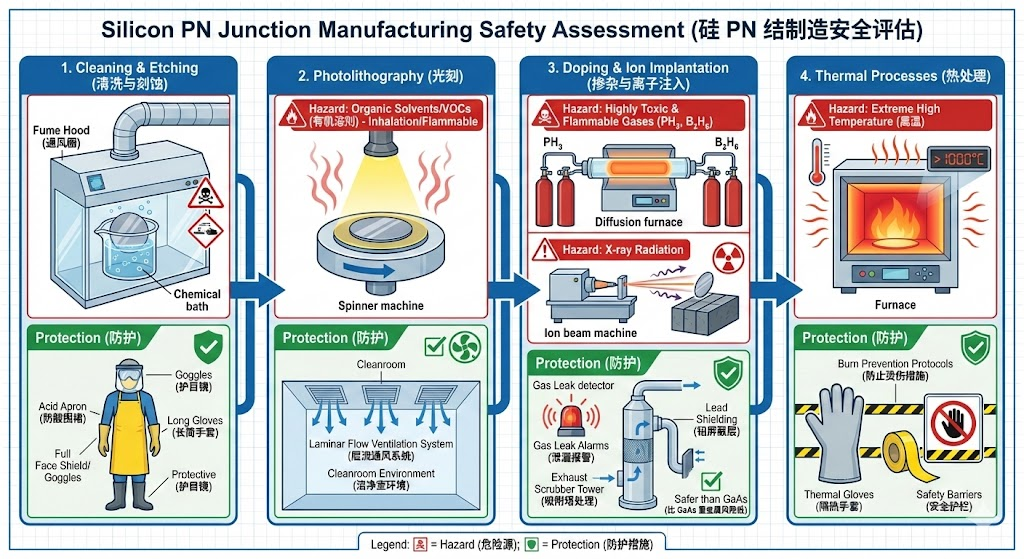
\includegraphics[width=1\textwidth]{p2.jpg}
\caption{制造安全评估}
\label{fig:p2}
\end{figure}

\subsection{社会与环境因素考量}

本设计方案的选择对社会可持续发展和环境保护具有积极意义。

\subsubsection{资源可持续性}

本设计选用的硅是地壳中含量第二丰富的元素，原料（石英砂）来源广泛且廉价。相比于储量稀缺且被列为战略资源的镓（Ga）和锗（Ge），硅基器件的大规模生产不会导致资源枯竭，符合可持续发展的工业理念。

\subsubsection{环境友好性}

{\heiti 低毒性废弃物：}

与GaAs等化合物半导体相比，硅基芯片在报废处理时不会释放砷等重金属污染物，降低了电子垃圾（E-waste）处理的难度和环境负荷。

{\heiti 能效贡献：}

本设计实现了极低的反向漏电流（pA级），若应用于大规模集成电路中，将显著降低待机功耗。这直接响应了国家"双碳"战略中对于电子产品节能降耗的要求。

\subsubsection{社会经济效益}

硅工艺（CMOS工艺）是目前全球最成熟、成本最低的半导体工艺。采用硅材料设计保证了该PN结可以利用现有的标准产线进行流片，无需定制昂贵的化合物半导体设备，从而大幅降低了制造成本，有利于产品的市场化推广和普及。

\begin{figure}[H]
\centering
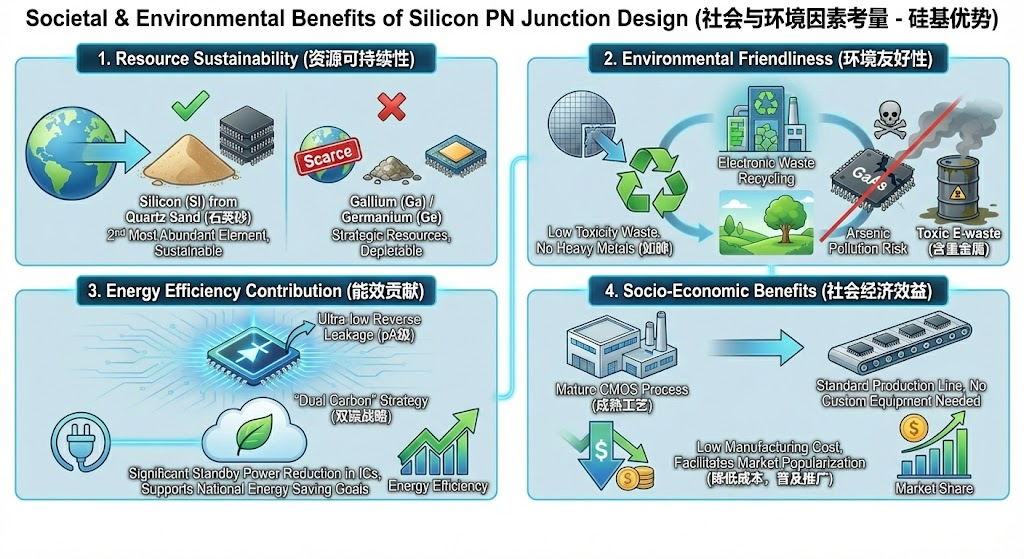
\includegraphics[width=1\textwidth]{p3.jpg}
\caption{社会与环境因素考量}
\label{fig:p3}
\end{figure}

\clearpage
\section{总结}

本报告针对 $T = 300\,\text{K}$ 工作温度下的 pn 结设计需求，通过系统的材料选择、参数设计和综合评估，最终确定了一套完整且可靠的设计方案。

在材料选择阶段，通过对 Ge、GaAs 和 Si 三种候选材料的开启电压、漏电流特性、少数载流子寿命以及结电容可实现性的多维度对比分析，确定硅（Si）为最优材料，其在满足所有技术指标的同时，兼具工艺成熟度高、成本低廉和环境友好等优势。

在参数设计阶段，基于电流对称性确定了掺杂比例 $N_A/N_D = 1.677$，并通过数值求解超越方程得到设计窗口 $6.180 \times 10^{12}\,\text{cm}^{-3} < N_D < 2.720 \times 10^{14}\,\text{cm}^{-3}$，最终选定 $N_D = 2.00 \times 10^{14}\,\text{cm}^{-3}$ 和 $N_A = 3.354 \times 10^{14}\,\text{cm}^{-3}$。所有验证结果表明该设计完全满足开启电压（$0.511\,\text{V} < 0.800\,\text{V}$）、电流对称性（$J_p = J_n = 1.072 \times 10^{-6}\,\text{A/cm}^2$）、反偏结电容（$1.374 \times 10^{-9}\,\text{F/cm}^2 < 1.60 \times 10^{-9}\,\text{F/cm}^2$）和反向漏电流（$4.017 \times 10^{-10}\,\text{A/cm}^2 < 1.30 \times 10^{-8}\,\text{A/cm}^2$）四项技术指标。

在设计评估阶段，从工程鲁棒性、生产安全和社会环境影响三个维度进行了深入分析，设计保留了 26\% 的上限余量和 44 倍的设计窗口宽度，确保了在实际工艺偏差下的高良率；同时，硅材料相比 GaAs 显著降低了生产过程中的毒性风险，且其资源丰富、可回收性强、能耗低的特点完全符合可持续发展理念。

综上所述，本设计方案在技术性能、工艺可行性、经济成本和社会责任之间实现了最优平衡，为后续的器件制造和工程应用奠定了坚实的理论基础。

\end{document}